\chapter{Pendolo su carrello}\label{PendCarrello}
\section{Modello e relative Equazioni}

\begin{figure}[ht]
	\centering
	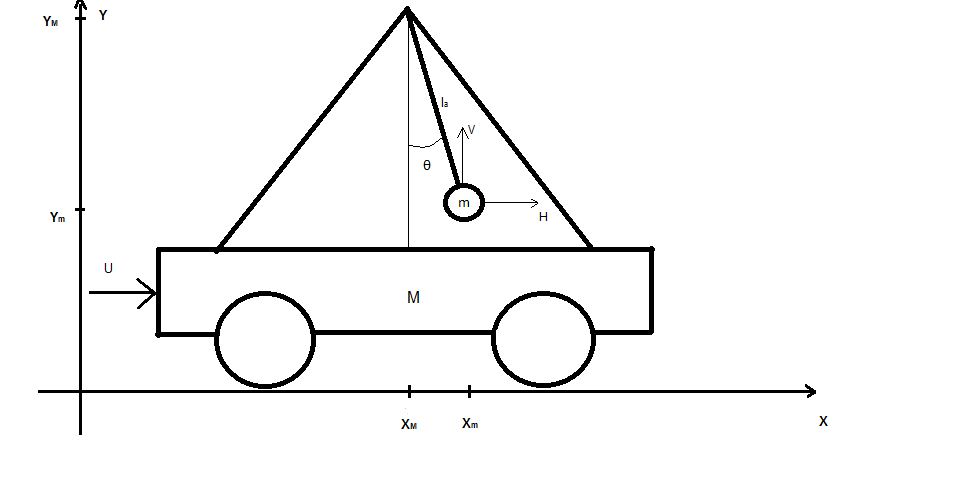
\includegraphics[width=\textwidth]{pendolo.png}\\
	\caption{Modello del pendolo su carrello}
	\label{pendolo}
\end{figure}
\textbf{Bilanciamento forze sull'asta}\\
Asse X:
\begin{equation}\notag
m\ddot{x}_m=H
\end{equation}
Asse Y:
\begin{equation}\notag
m\ddot{y}_m=V-mg
\end{equation}
Dove $H$ e $V$ sono le reazioni vincolari (orizzontale e verticale) a cui e sottoposta la massa $m$ per il fatto di essere bloccata all'estremità dell'asta.\\ 
Essendo:\\
\begin{equation}\notag
x_m = x_M+l_a\sin(\theta) \quad \Rightarrow \quad \ddot{x}_m=\ddot{x}_M-l_a\sin(\theta)\dot{\theta}^2+l_a\cos(\theta)\ddot{\theta}
\end{equation}
\begin{equation}\notag
y_m=y_M-l_a\cos(\theta) \quad \Rightarrow \quad \ddot{y}_m=l_a\sin(\theta)\ddot{\theta}+l_a\cos(\theta)\dot{\theta}^2
\end{equation}
Si ottiene:
\begin{equation}\label{Hv}
H=m\ddot{x}_M-ml_a\sin(\theta)\dot{\theta}^2+ml_a\cos(\theta)\ddot{\theta}
\end{equation}
\begin{equation}\label{Vv}
V=mg+ml_a\cos(\theta)\dot{\theta}^2+ml_a\sin(\theta)\ddot{\theta}
\end{equation}
\textbf{Bilanciamento forze sul carrello}
\begin{equation}\notag
M\ddot{x}_M=u-H
\end{equation}
sostituendo la \ref{Hv} si ha:
$$
M\ddot{x}_M=u-m\ddot{x}_M+ml_a\sin(\theta)\dot{\theta}^2-ml_a\cos(\theta)\ddot{\theta}
$$
\begin{equation}\label{FCarr}
(M+m)\ddot{x}_M+ml_a\cos(\theta)\ddot{\theta}=u+ml_a\dot{\theta}^2\sin(\theta)
\end{equation} 
\textbf{Bilanciamento momenti del sistema asta-massa}
\begin{equation}
I_m\ddot{\theta}=l_aV\sin(\theta)+l_aH\cos(\theta)
\end{equation}
sostituendo la \ref{Hv} e la \ref{Vv}:
$$
I_m\ddot{\theta}=l_a\sin(\theta)[mg+ml_a\cos(\theta)\dot{\theta}^2+ml_a\sin(\theta)\ddot{\theta}]+$$$$+l_a\cos(\theta)[m\ddot{x}_M-ml_a\sin(\theta)\dot{\theta}^2+ml_a\cos(\theta)\ddot{\theta}]=
$$
$$
=mgl_a\sin(\theta)+ml_a^2\sin(\theta)\cos(\theta)\dot{\theta}^2+ml_a^2\sin^2(\theta)\ddot{\theta}+ml_a\ddot{x}_M\cos(\theta)+$$$$-ml_a^2\cos(\theta)\sin(\theta)\dot{\theta}^2
+ml_a^2\cos^2(\theta)\ddot{\theta}=$$
$$=mgl_a\sin(\theta)+ml_a^2\ddot{\theta}+ml_a\ddot{x}_M\cos(\theta) =
$$
\begin{equation} \label{momInThetaP}
=ml_a(g\sin(\theta)+l_a\ddot{\theta}+\ddot{x}_M\cos(\theta))
\end{equation}
Essendo il momento d'inerzia dell'asta molto inferiore rispetto a quello della massa $m$ attaccata al pendolo, possiamo per semplicità trascurarlo, per cui poniamo $I_m=0$. Vedremo poi nel paragrafo \ref{Im} che i risultati senza approssimazione saranno praticamente gli stessi.\\
Il sistema che deriva dalla \ref{FCarr} e dalla \ref{momInThetaP} è dunque il seguente:
\\\\
$\begin{cases}
$$(M+m)\ddot{x}_M+ml_a\cos(\theta)\ddot{\theta}=u+ml_a\dot{\theta}^2\sin(\theta)$$ \\
$$g\sin(\theta)+l_a\ddot{\theta}+\ddot{x}_M\cos(\theta)=0$$\\
\end{cases}
$
\\\\
Dalla prima equazione del sistema 
$$
(M+m)(\frac{-g\sin(\theta)-l_a\ddot{\theta}}{\cos(\theta)})+ml_a\cos(\theta)\ddot{\theta}=u+ml_a\dot{\theta}^2\sin(\theta)
$$
$$
\ddot{\theta}(ml_a\cos(\theta)-\frac{l_a(M+m)}{\cos(\theta)}=u+ml_a\dot{\theta}^2\sin(\theta)+\frac{g\sin(\theta)(M+m)}{\cos(\theta)}
$$
$$
\ddot{\theta}=\frac{[u+ml_a\dot{\theta}^2\sin(\theta)+\displaystyle\frac{g\sin(\theta)(M+m)}{\cos(\theta)}]\cos(\theta)}{ml_a\cos^2(\theta)-l_a(M+m)} \Rightarrow$$\\
\begin{equation}\label{theta2punti}
\ddot{\theta}=\frac{u\cos(\theta)+ml_a\dot{\theta}^2\sin(\theta)\cos(\theta)+g\sin(\theta)(M+m)}{-l_a(m\sin^2(\theta)+M)}
\end{equation}\\
Dalla seconda equazione del sistema
$$
\ddot{x}_M=\frac{-g\sin(\theta)-l_a\ddot{\theta}}{\cos(\theta)}
$$
e sostituendo ora la \ref{theta2punti}  
$$
\ddot{x}_M=\frac{-g\sin(\theta)-\displaystyle\frac{ul_a\cos(\theta)+ml^2_a\dot{\theta}^2\sin(\theta)\cos(\theta)+gl_a\sin(\theta)(M+m)}{-l_a(m\sin^2(\theta)+M)}}{\cos(\theta)}=
$$
$$
=\frac{g\sin(\theta)[-l_a(m\sin^2(\theta)+M)]+ul_a\cos(\theta)+ml^2_a\dot{\theta}^2\sin(\theta)\cos(\theta)+gl_a\sin(\theta)(M+m)}{l_a\cos(\theta)(m\sin^2(\theta)+M)}=
$$
$$
=\frac{-gm\sin^3(\theta)-gM\sin(\theta)+u\cos(\theta)+ml_a\dot{\theta}^2\sin(\theta)\cos(\theta)+gM\sin(\theta)+gm\sin(\theta)}{\cos(\theta)(m\sin^2(\theta)+M)}
$$
$$
=\frac{u+ml_a\dot{\theta}^2\sin(\theta)+gm\cos(\theta)\sin(\theta)}{m\sin^2(\theta)+M}
$$\\
Assegniamo le variabili di stato e definiamo le uscite desiderate:\\\\
$\begin{cases}
$$x_1 \stackrel{\Delta}{=} x_M$$ \\
$$x_2\stackrel{\Delta}{=}\dot{x}_M$$\\
$$x_3\stackrel{\Delta}{=}\theta$$\\
$$x_4\stackrel{\Delta}{=}\dot{\theta}$$\\
$$y_1\stackrel{\Delta}{=}x_M$$ \\
$$y_2\stackrel{\Delta}{=}\theta$$\\
\end{cases}
$\\\\\\
Sostituendo queste ultime nelle equazioni appena ricavate si ottengono le equazioni:
\\\\\\
$\underline{\dot{x}}=\displaystyle\frac{d}{d t}
\begin{bmatrix}
x_M\\\\
\dot{x}_M\\\\
\theta\\\\
\dot{\theta}\\\\
\end{bmatrix}
=
\begin{bmatrix}
x_2\\\\
\displaystyle\frac{u+ml_ax_4^2\sin(x_3)+gm\cos(x_3)\sin(x_3)}{m\sin^2(x_3)+M}\\\\
x_4\\\\
-\displaystyle\frac{u\cos(x_3)+ml_ax_4^2\sin(x_3)\cos(x_3)+g(M+m)\sin(x_3)}{l_a(m\sin^2(x_3)+M)}\\\\
\end{bmatrix}
$
\\\\\\
\section{Linearizzazione del modello}\label{LinMod}
\textbf{Punti di equilibrio del sistema} \\
Per la ricerca dei punti di equilibrio poniamo $\underline{f}(\underline{x},u)=\underline{0}$\quad(dove $\underline{\dot{x}}=\underline{f}(\underline{x},u$)):\\\\
$\begin{cases}
$$x_2=0$$ \\
$$\displaystyle\frac{u+ml_ax_4^2\sin(x_3)+gm\cos(x_3)\sin(x_3)}{m\sin^2(x_3)+M}=0$$\\
$$x_4=0$$\\
$$\displaystyle\frac{u\cos(x_3)+ml_ax_4^2\sin(x_3)\cos(x_3)+g(M+m)\sin(x_3)}{l_a(m\sin^2(x_3)+M)}=0$$
\end{cases}
$\\\\\\
Dal precedente sistema si capisce che punti di equilibrio del pendolo su carrello sono due, uno instabile per \\
$\begin{cases}
$$x_1=\forall$$ \\
$$x_2=0$$\\
$$x_3=\pm\pi$$\\
$$x_4=0$$\\
$$u=0$$
\end{cases}$\\
ovvero quando il pendolo è rivolto verso l'alto (pendolo inverso), l'altro, stabile, per\\
$\begin{cases}
$$x_1=\forall$$ \\
$$x_2=0$$\\
$$x_3=0$$\\
$$x_4=0$$\\
$$u=0$$
\end{cases}$\\
quando il pendolo è rivolto verso il basso (pendolo "normale").
Siccome il punto di equilibrio non dipende dalla posizione del carrello possiamo per semplicità scegliere $x_1=0$.\\\\
\textbf{Linearizzazione del sistema attorno al punto di equilibrio}\\
Vogliamo ora linearizzare le precedenti equazioni di stato attorno al punto di equilibrio $\underline{\tilde{x}}=\underline{0}$, $\tilde{u}=0$ trovato: \\\\
$\displaystyle\frac{\partial{f_1}}{\partial{\underline{x}}}(\underline x,u)=
\begin{bmatrix}
0&1&0&0
\end{bmatrix}$\qquad
$\displaystyle\frac{\partial{f_1}}{\partial{u}}(\underline{x},u)=0$\\\\\\
$\displaystyle\frac{\partial{f_2}}{\partial{x_1}}(\underline{x},u)=0$\qquad
$\displaystyle\frac{\partial{f_2}}{\partial{x_2}}(\underline{x},u)=0$\\
$\displaystyle\frac{\partial{f_2}}{\partial{x_3}}(\underline{x},u)=\displaystyle\frac{[ml_ax_4^2\cos(x_3)+mg(\cos^2(x_3)-\sin^2(x_3))](M+m\sin^2(x_3))}{(M+m\sin^2(x_3))^2}$\\
$-\displaystyle\frac{[u+ml_ax_4^2\sin(x_3)+mg\sin(x_3)\cos(x_3)](2\sin(x_3)\cos(x_3))}{(M+m\sin^2(x_3))^2}\bigg|_{\underline{\tilde{x}},\tilde{u}}=\displaystyle\frac{mg}{M}$\\ $\displaystyle\frac{\partial{f_2}}{\partial{x_4}}(\underline{x},u)=\displaystyle\frac{2ml_a\sin(x_3)x_4}{M+m\sin^2(x_3)}\bigg|_{\underline{\tilde{x}},\tilde{u}}=0$\quad$\displaystyle\frac{\partial{f_2}}{\partial{u}}(\underline{x},u)=\displaystyle\frac{1}{M+m\sin^2(x_3)}\bigg|_{\underline{\tilde{x}},\tilde{u}}=\displaystyle\frac{1}{M}$\\\\\\
$\displaystyle\frac{\partial{f_3}}{\partial{\underline{x}}}(\underline x,u)=
\begin{bmatrix}
0&0&0&1
\end{bmatrix}$\qquad$\displaystyle\frac{\partial{f_3}}{\partial{u}}(\underline{x},u)=0$\\\\\\
$\displaystyle\frac{\partial{f_4}}{\partial{x_1}}(\underline{x},u)=0$\qquad
$\displaystyle\frac{\partial{f_4}}{\partial{x_2}}(\underline{x},u)=0$\\
$\displaystyle\frac{\partial{f_4}}{\partial{x_3}}(\underline{x},u)=\displaystyle\frac{[u\sin(x_3)-ml_ax_4^2(\cos^2(x_3)-\sin^2(x_3))-g\cos(x_3)(M+m)][l_a(m\sin^2(x_3)+M)]}{l_a^2(m\sin^2(x_3)+M)^2}+$ $-\displaystyle\frac{[-u\cos(x_3)-ml_ax^2_4\sin(x_3)\cos(x_3)-g\sin(x_3)(m+M)][2ml_a\sin(x_3)\cos(x_3)]}{l_a^2(m\sin^2(x_3)+M)^2}\bigg|_{\underline{\tilde{x}},\tilde{u}}=$
$=-\displaystyle\frac{(M+m)g}{Ml}$\qquad$\displaystyle\frac{\partial{f_4}}{\partial{x_4}}(\underline{x},u)=\displaystyle\frac{-2ml_ax_4\sin(x_3)\cos(x_3)}{l_a(m\sin^2(x_3)+M)}\bigg|_{\underline{\tilde{x}},\tilde{u}}=0$\\$\displaystyle\frac{\partial{f_4}}{\partial{u}}(\underline{x},u)=\displaystyle\frac{-\cos(x_3)}{l_a(m\sin^2(x_3)+M)}\bigg|_{\underline{\tilde{x}},\tilde{u}}=-\displaystyle\frac{1}{ml_a}$\\\\\\
Le equazioni linearizzate sono dunque:\\\\
$\underline{\delta\dot{x}}=
\begin{bmatrix}
0&1&0&0\\
0&0&\displaystyle\frac{mg}{M}&0\\
0&0&0&1\\
0&0&-\displaystyle\frac{(M+m)g}{Ml_a}&0
\end{bmatrix}
\underline{\delta x}+
\begin{bmatrix}
0\\
\displaystyle\frac{1}{M}\\
0\\
-\displaystyle\frac{1}{Ml_a}\\
\end{bmatrix}
\underline{\delta u}
$\\\\
$\underline{\delta y}=
\begin{bmatrix}
1&0&0&0\\
0&0&1&0
\end{bmatrix}
\underline{\delta x}
$\\\\\\
Calcolando ora la funzione di trasferimento $T(s)$ tra l'ingresso $u$ (forza esercitata sul carrello,
avanti/indietro) e l'uscita $y_2$(angolo $\theta$ del pendolo rispetto alla verticale) si ottiene:\\\\
$T_{y_2,u}(s)=C(sI-A)^{-1}B=
\begin{bmatrix}
0&0&1&0
\end{bmatrix}
\begin{bmatrix}
*&*&*&*\\
*&*&*&*\\
*&0&*&\displaystyle\frac{1}{s^2+\frac{(M+m)g}{Ml_a}}\\
*&*&*&*
\end{bmatrix}
\begin{bmatrix}
0\\
\displaystyle\frac{1}{M}\\
0\\
-\displaystyle\frac{1}{Ml_a}\\
\end{bmatrix} = \\
=-\displaystyle\frac{1}{Ml_as^2+(M+m)g}
$\\\\\\
Inserendo ora i parametri del modello fisico del pendolo su  carrello realizzato con l'ausilio del Lego MINDSTORM EV3 si può procedere all'identificazione della funzione di trasferimento\\\\
\begin{tabular}{|l|l|l|}
	\hline
	\textbf{Parametro} & \textbf{Valore} & \textbf{Unità di misura}\\
	\hline
	$M$ & 0.7535 & $kg$\\
	\hline
	$m$ & 0.015 & $kg$ \\
	\hline
	$g$ & 9.81 & $m/s^2$\\
	\hline
	$l_a$ & 0.166 & $m$\\
	\hline
\end{tabular}\\\\\\
Data la precedente tabella si ha:\\
$T_{y_2,u}(s)=-\displaystyle\frac{1}{0.125s^2+7.539}$
\newpage
\section{Stabilizzazione del pendolo}
Il pendolo di per sè è un sistema già stabile, lo scopo della realizzazione su carrello consiste nello smorzarne l'oscillazione riducendo la costante di tempo del sistema grazie all'impiego di due ruote motrici.\\
In figura \ref{pendoloFisico} realizzazione del pendolo su carrello utilizzando un motore EV3 Large Servo Motor come trazione e un encoder GlideWheel-M per misurare l'angolo del pendolo 
\begin{figure}[ht]
	\centering
	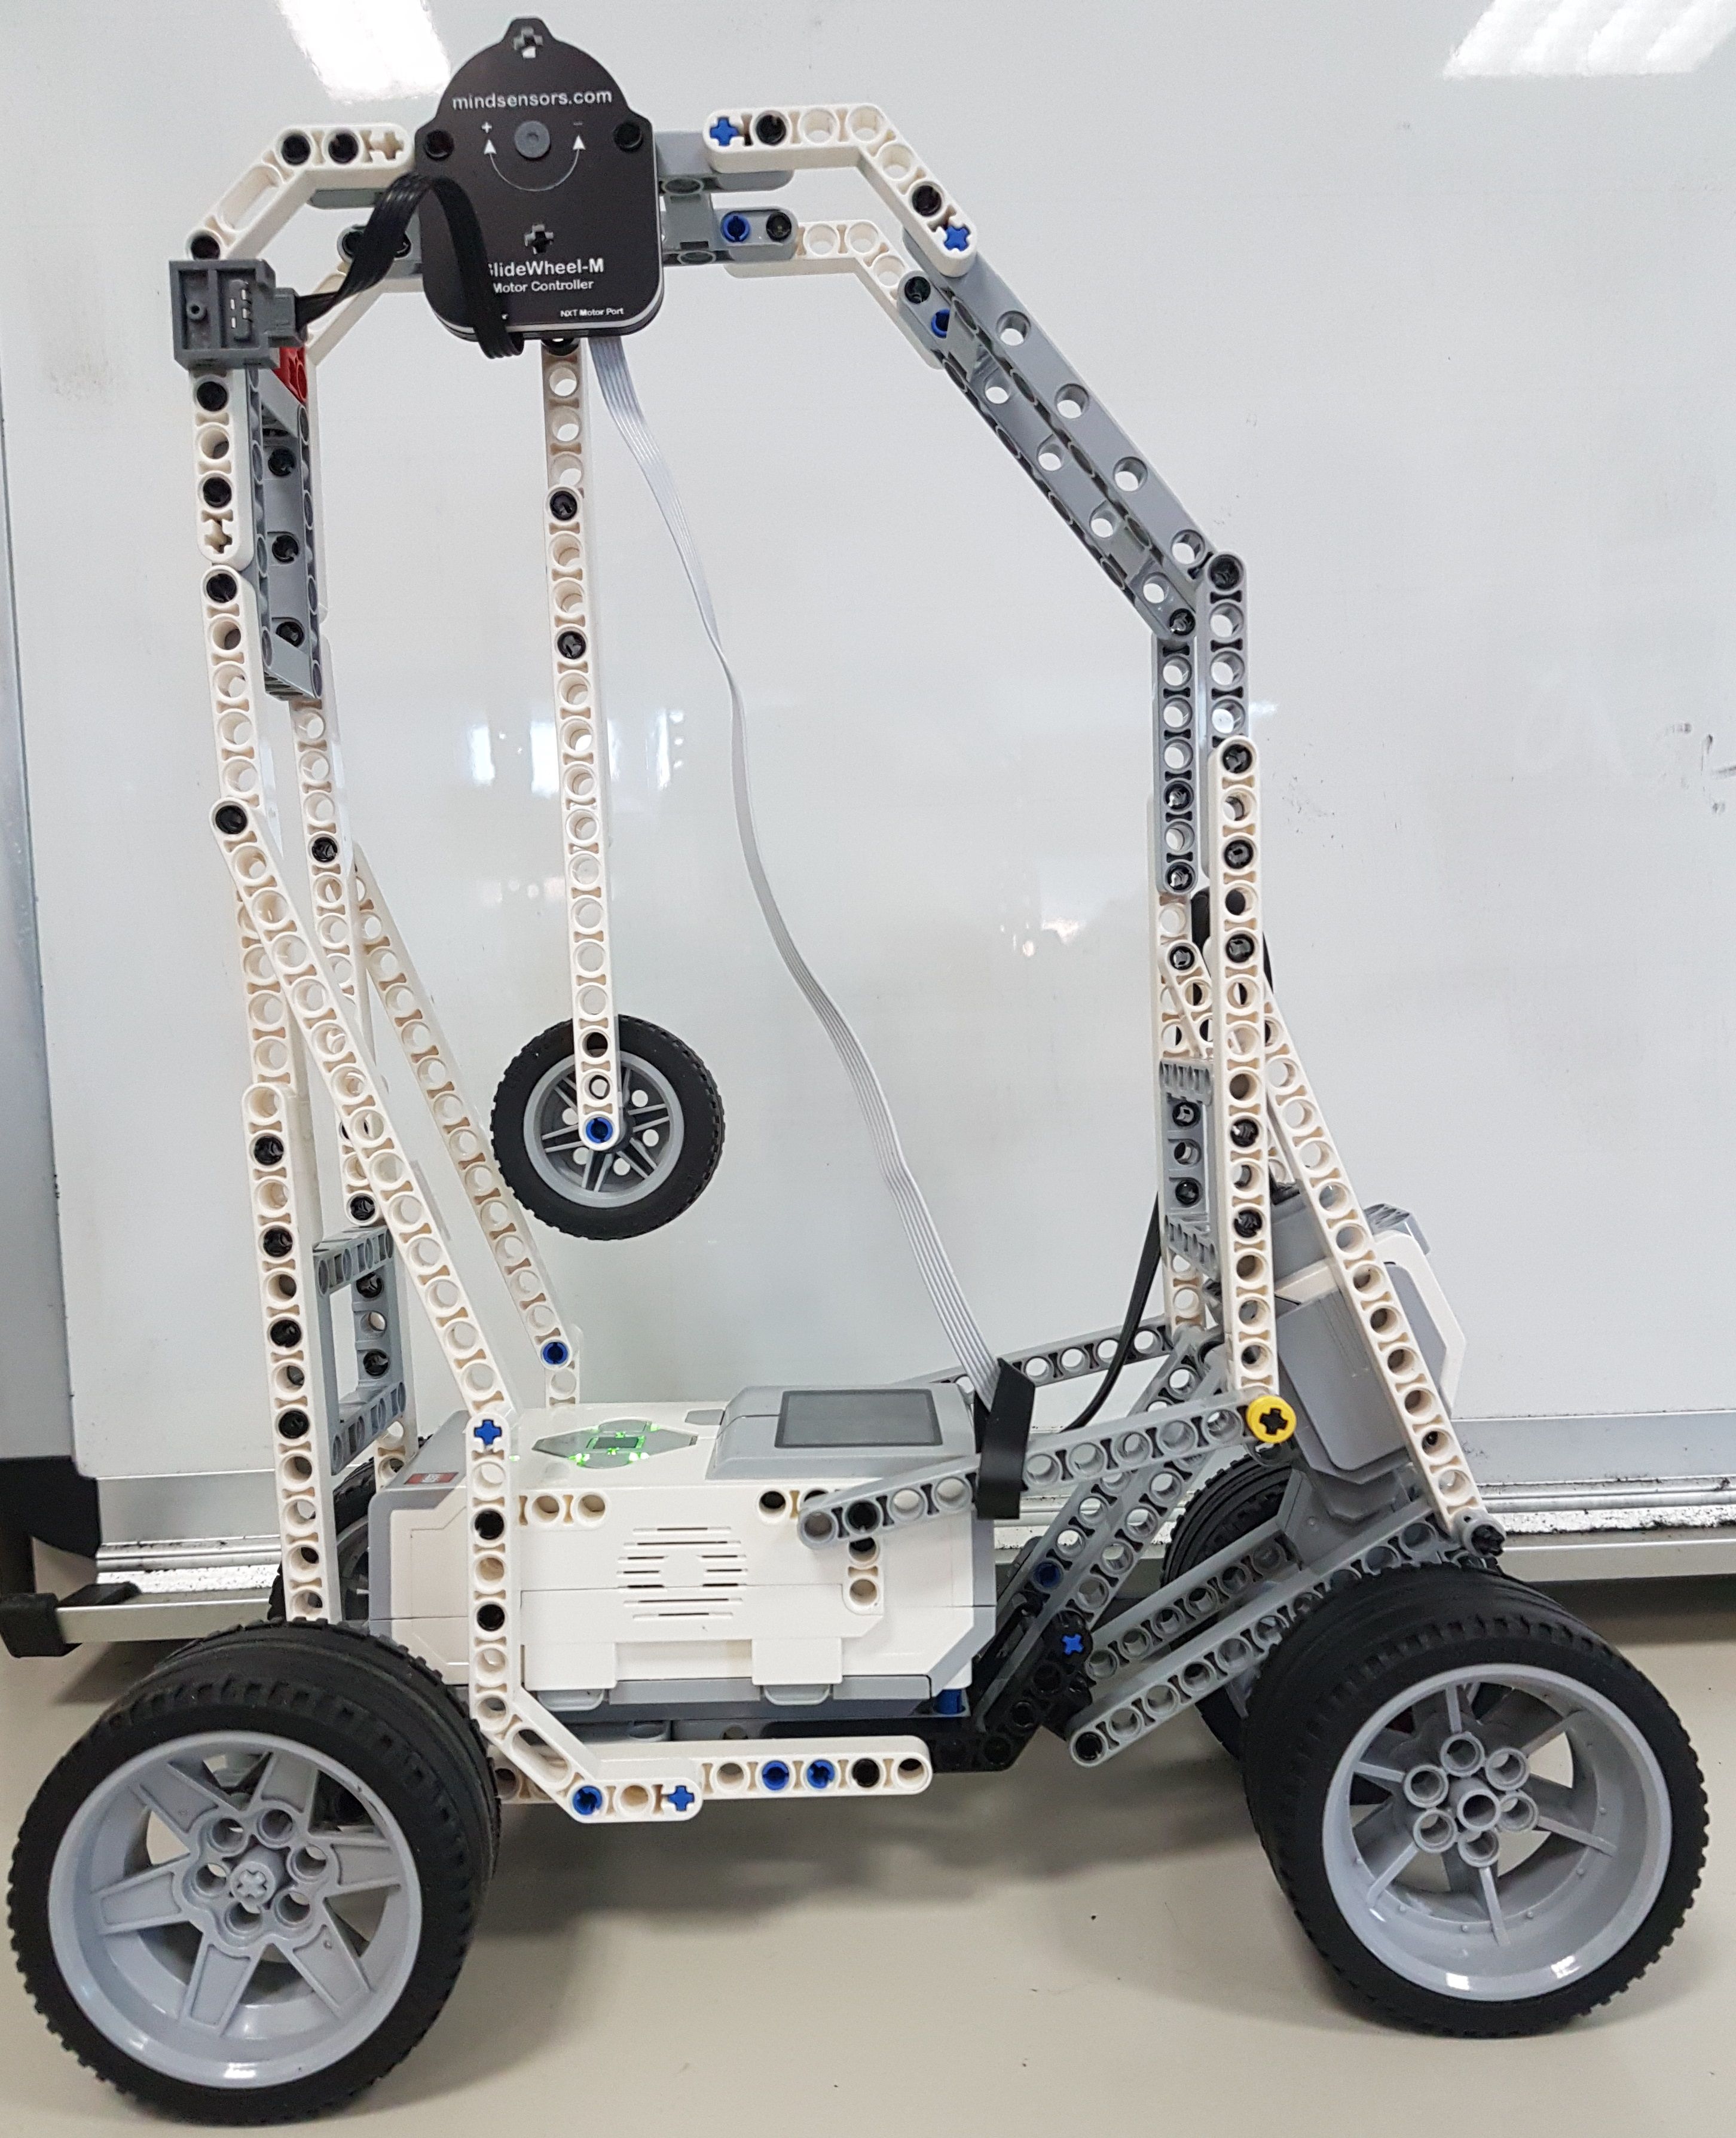
\includegraphics[scale=0.08]{pendoloFisico.jpg}\\
	\caption{Realizzazione fisica del pendolo su carrello}
	\label{pendoloFisico}
\end{figure} 
rispetto alla verticale.\\
Da specifiche quest'ultimo può raggiungere un tempo di campionamento minimo di 0.001s (così come il motore) ma a tale valore non riesce sempre a campionare in modo corretto, perciò abbiamo deciso di aumentarlo in modo da non perdere nessuna variazione anche alla massima velocità angolare raggiunta dal pendolo durante l'oscillazione libera tra $[\ang{-31},\ang{+31}]$ (intervallo entro il quale il pendolo è vincolato per costruzione).
\begin{figure}[ht]
	\centering
	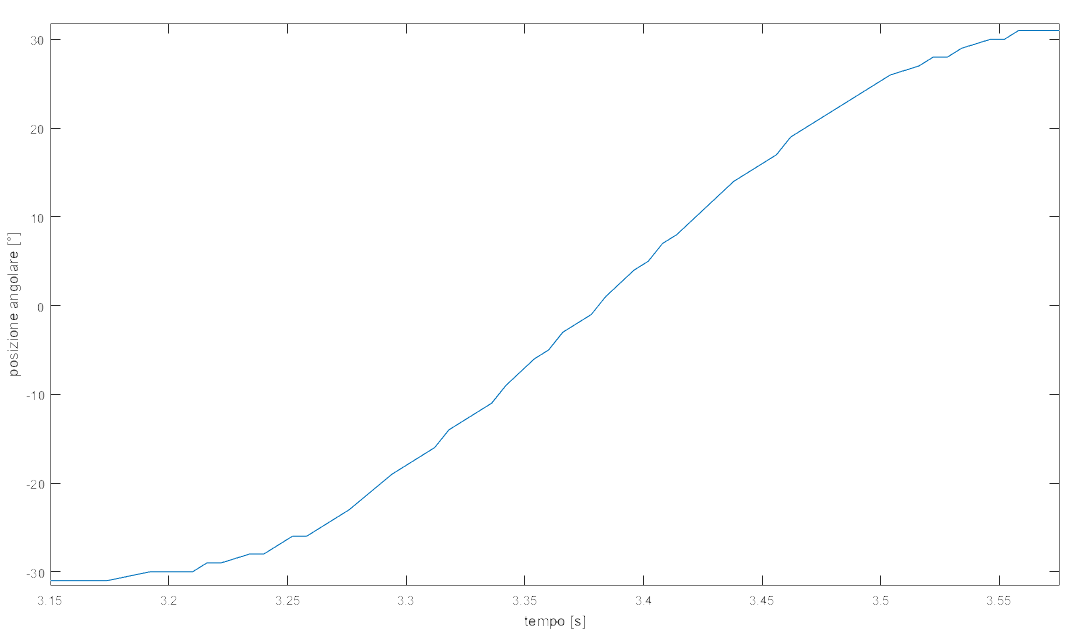
\includegraphics[scale=0.4]{SlewRate.PNG}\\
	\caption{Massima velocità di oscillazione libera}
	\label{slewRate}
\end{figure}
Da tale esperimento è risultato che durante la prima oscillazione (in figura \ref{slewRate}), il pendolo, raggiunge per $\theta=\ang{0}$ la velocità $\omega=250\frac{\deg}{s}$(calcolata con un semplice rapporto incrementale) per cui il tempo di campionamento ottimale sarebbe stato $t_c=\displaystyle\frac{1}{250}=0.004s$.
Sfruttando il modello del motore LEGO da noi ricavato si può quindi ricavare la funzione di Trasferimento del sistema complessivo (avente come ingresso la potenza richiesta al motore e come uscita la posizione angolare del pendolo).\\
Siccome in uscita al modello del motore abbiamo la coppia erogata dallo stesso, per poterlo mettere in serie al modello del pendolo su carrello (il quale come ingresso riceve una spinta sotto forma di forza) occorre adattare il collegamento I/O. Poiché si assume un puro moto di rotolamento delle ruote del carrello si tratta di trovare il giusto coefficiente di proporzionalità tra coppia e spinta.
Abbiamo verificato sperimentalmente con la sovrapposizione dei grafici simulati in Simulink e quelli reali del sistema complessivo ottenuti dalla misura dei sensori MINDSTORM che tale coefficiente risulta essere all'incirca $17$.
\begin{figure}[ht]
	\centering
	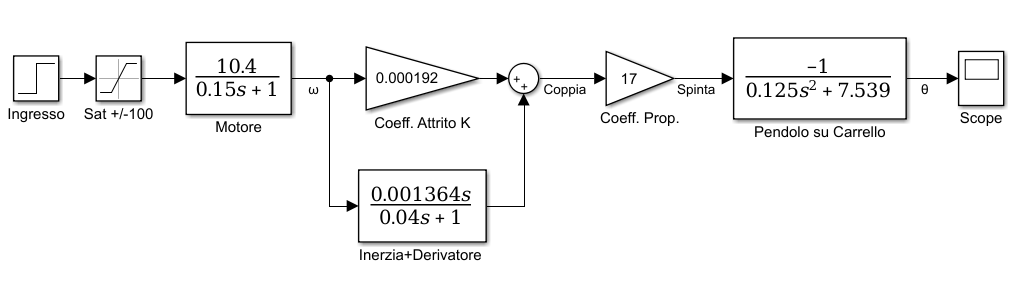
\includegraphics[width=\textwidth]{SisComplessivoPendoloNormale.PNG}
	\caption{Schema a blocchi del sistema complessivo}
	\label{SisComplessivoPendoloNormale}
\end{figure}
Per realizzare ora una retroazione algebrica sull'uscita che ci permetta di controllarlo in ciclo chiuso, possiamo riassumere in un'unica funzione di Trasferimento il sistema complessivo:\\
$$T_{y_2,u}=-\displaystyle\frac{323.4s+45.26}{s^4+31.67s^3+227s^2+1910s+10050}$$\\
della quale si può calcolare il luogo delle radici per studiarne la stabilità in ciclo chiuso.
\begin{figure}[ht]
	\centering
	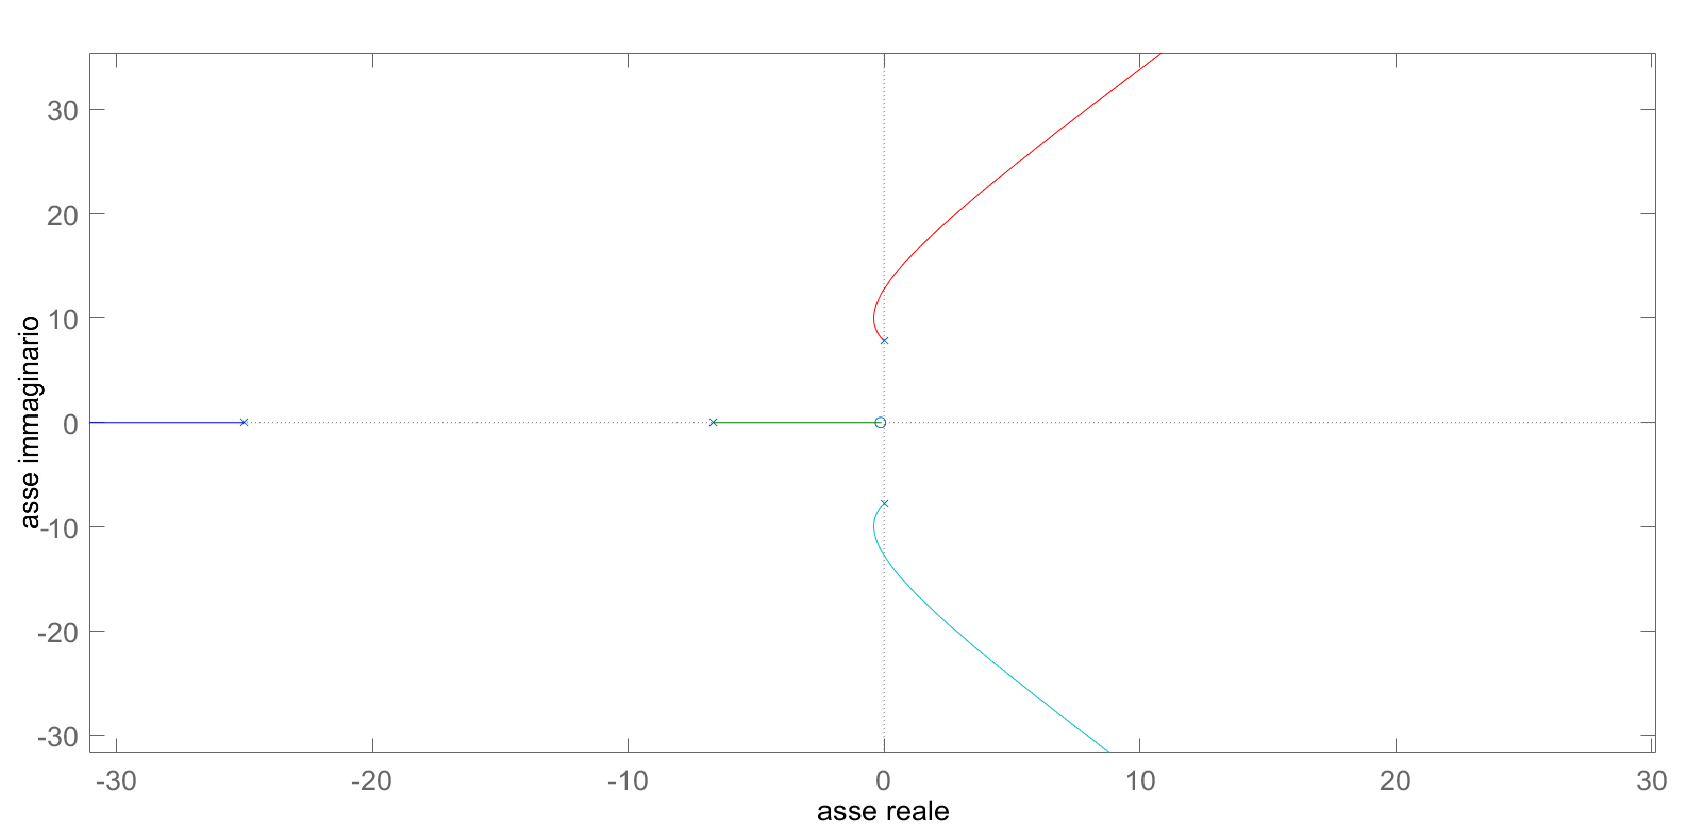
\includegraphics[width=\textwidth]{RLocusPendoloNormale.PNG}
	\caption{Luogo delle Radici di $-T_{y_2,u}$}
	\label{RLocusPendoloNormale}
\end{figure}
Come si evince dal luogo delle radici del sistema, è possibile utilizzare un semplice Regolatore Proporzionale purché il suo guadagno rientri in un intervallo molto limitato ovvero $P\in(-10,0)$.\\
Attraverso l'utilizzo di uno strumento MATLAB quale `sisotool' e grazie ad un'analisi sperimentale siamo arrivati a definirne il 
\begin{figure}[ht]
	\centering
	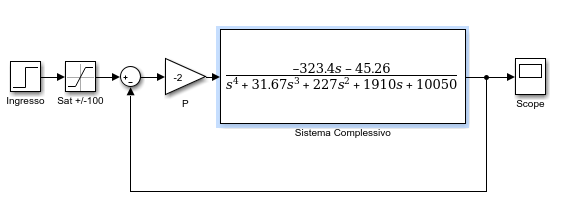
\includegraphics[width=\textwidth]{SisComplessivoPNRetroazionato.PNG}
	\caption{Sistema complessivo controllato proporzionalmente}
	\label{SisComplessivoPNRetroazionato}
\end{figure}
guadagno $P=-2$.\\
Il Regolatore proporzionale permette di ridurre ampiamente il periodo di oscillazione del pendolo.\\
Abbiamo quindi sperimentato e osservato il comportamento del sistema cercando di quantificare il miglioramento 
\begin{figure}[ht]
	\centering
	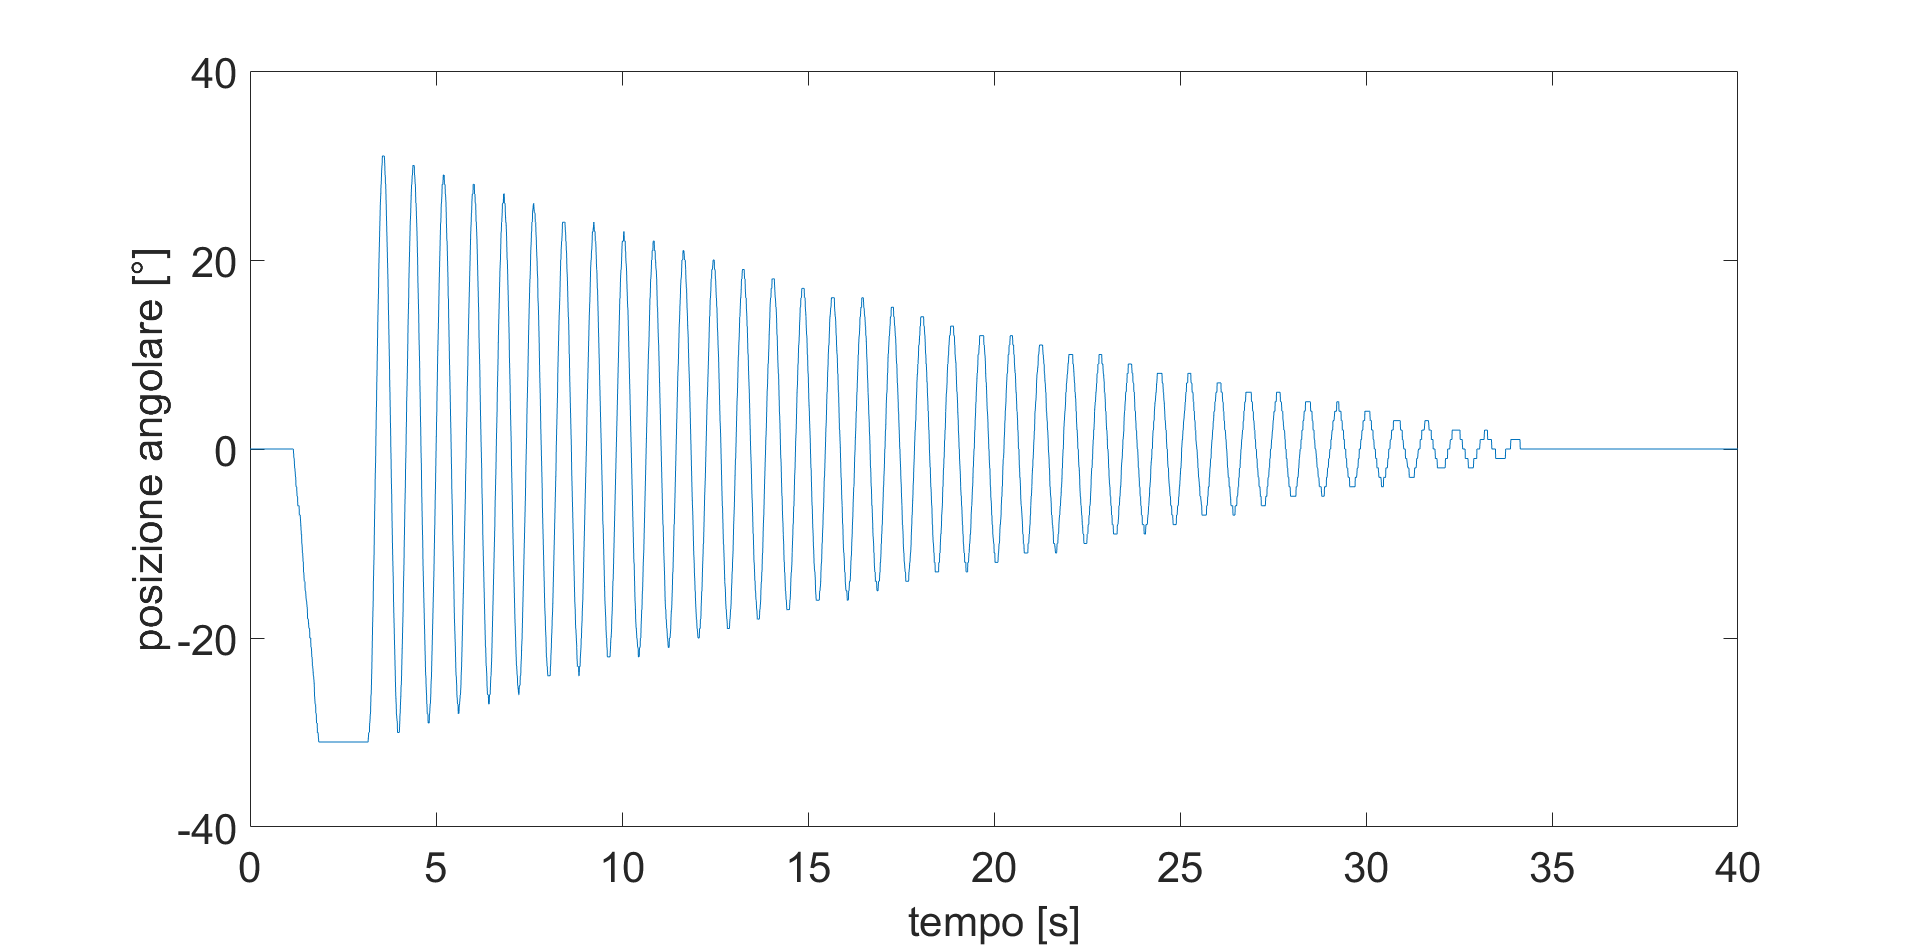
\includegraphics[scale=0.402]{oscillOL.PNG}
	\caption{Sistema in ciclo aperto}
	\label{oscillOL}
\end{figure} 
ottenuto.\\
Come si può vedere nel grafico in figura \ref{oscillOL} posizionando il pendolo ad un'angolazione iniziale di $\theta=\ang{31}$, in ciclo aperto(ovvero senza controllo sul motore) si raggiunge il punto di stabilità $\theta=\ang{0}$ in poco più di 30 secondi, mentre risulta un tempo di appena 1.4 secondi per quanto riguarda il sistema 
\begin{figure}[ht]
	\centering
	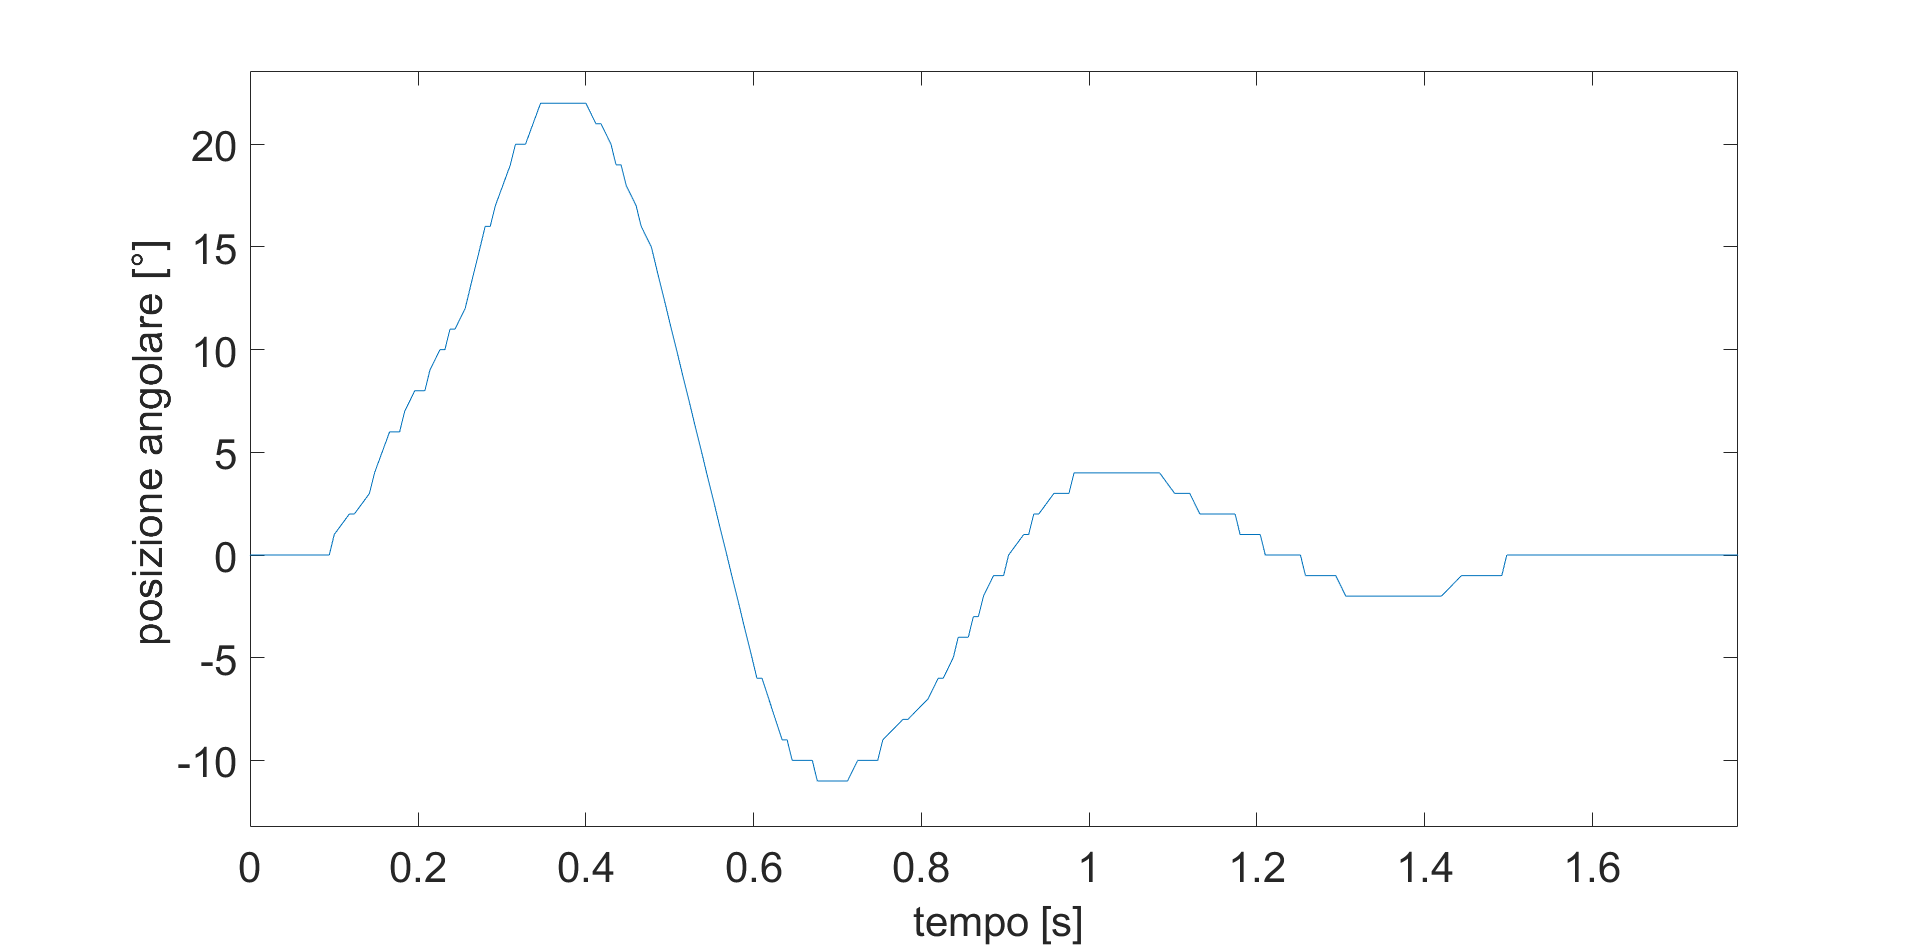
\includegraphics[scale=0.402]{oscillCL.PNG}
	\caption{Sistema in ciclo chiuso con Regolatore P}
	\label{oscillCL}
\end{figure}
in ciclo chiuso.\\
Un Regolatore migliore potrebbe essere un PID (Proporzionale Integrativo Derivativo) che permette grazie all'aggiunta di uno zero ($\in\Re$), e quindi necessariamente almeno un polo ($\in\Re$) di avere un maggiore margine di stabilità.
\section{Controllo della posizione del carrello}
Fino ad ora abbiamo trascurato la seconda uscita di nostro interesse, ovvero la posizione del carrello
$x_M$. Perciò vogliamo provare a controllare quest'ultima in modo da decidere non solo il tempo di assestamento del pendolo ma allo stesso tempo anche la posizione del carrello dove il sistema dovrà assestarsi.\\
A tal proposito riprendiamo le equazioni ricavate al paragrafo \ref{LinMod}.\\
Dalle seguenti equazioni di stato linearizzate attorno al punto di equilibrio $\underline{x}=\underline{0}$, $u=0$\\\\
$\underline{\delta\dot{x}}=
\begin{bmatrix}
0&1&0&0\\
0&0&\displaystyle\frac{mg}{M}&0\\
0&0&0&1\\
0&0&-\displaystyle\frac{(M+m)g}{Ml_a}&0
\end{bmatrix}
\underline{\delta x}+
\begin{bmatrix}
0\\
\displaystyle\frac{1}{M}\\
0\\
-\displaystyle\frac{1}{Ml_a}\\
\end{bmatrix}
\underline{\delta u}
$\\\\
$\underline{\delta y}=
\begin{bmatrix}
1&0&0&0\\
0&0&1&0
\end{bmatrix}
\underline{\delta x}
$\\\\\\
si può ricavare la funzione di trasferimento $T_{y_1,u}(s)$ tra l'ingresso $u$ (forza esercitata sul carrello,
avanti/indietro) e l'uscita $y_1$(posizione $x_M$ del carrello):\\\\
$T_{y_1,u}(s)=
\begin{bmatrix}
1&0&0&0
\end{bmatrix}
\begin{bmatrix}
*&\displaystyle\frac{1}{s^2}&*&\displaystyle\frac{mg}{s^2(Ms^2+\displaystyle\frac{(m+M)g}{l_a})}\\
*&*&*&*\\
*&*&*&*\\
*&*&*&*
\end{bmatrix}
\begin{bmatrix}
0\\
\displaystyle\frac{1}{M}\\
0\\
-\displaystyle\frac{1}{Ml_a}\\
\end{bmatrix} = \\
=\displaystyle\frac{s^2+\displaystyle\frac{g}{l_a}}{s^2(Ms^2+\displaystyle\frac{(M+m)g}{l_a})}
$\\\\
Sostituendo i parametri del modello si ha:\\\\
$T_{y_1,u}(s)=\displaystyle\frac{1.327s^2+78.42}{s^2(s^2+60.27)}$
